\documentclass[11pt]{article}
%\renewcommand{\thesection}{\Roman{section}}  %zmiana section na rzymskie
\usepackage[utf8]{inputenc}
\usepackage[OT4]{polski}
\usepackage{tabularx}
\usepackage[margin=60pt]{geometry}
\usepackage{amsmath}
\usepackage{amsfonts}
\usepackage{listings} 
\usepackage[usenames,dvipsnames,table,xcdraw]{xcolor}
\usepackage{array}
\usepackage{sidecap} %do grafik
\usepackage{wrapfig} % j. w.
\usepackage{graphicx} %j.. w.
\usepackage{subfig} %j. w.
\usepackage{booktabs}
\usepackage{longtable}
\usepackage{hyperref}
\usepackage{nicefrac}
\usepackage{multirow}



\title{Komputerowa symulacja jednowymiarowego ruchu ciała z wykorzystaniem 
formalizmu Newtona.}

\author{Paweł Rzońca}

\begin{document}

\maketitle

\section*{Wstęp}
Wahadłem matematycznym określamy punktową masę zawieszoną na nierozciągliwej 
nici w jednorodnym polu grawitacyjnym. Rozwiązując je przy założeniu więzu na 
$R = $ const (masa na sztywnym, nieważkim, cienkim pręcie), sytuacja sprowadza się do ruchu jednowymiarowego opisywanego równaniem 
\begin{equation}\label{1}
R \ddot{\varphi} + g\sin \varphi=0, 
\end{equation}
gdzie $\varphi$ jest kątem pomiędzy kierunkiem pola grawitacyjnego a nicią.

Równanie to można rozwiązać analitycznie dla małych kątów, takich dla których 
zasadne jest przybliżenie 
$$\sin \varphi \simeq \varphi,$$
a samo równanie przyjmuje postać 
\begin{equation}
\ddot{\varphi} + \dfrac{g}{R} \varphi = 0.
\end{equation}
Rozwiązanie tego równania ma postać:
\begin{equation} \label{3}
\varphi (t) = A \sin ( \sqrt{g\/R} t +\alpha ),
\end{equation}
gdzie stałe $A$ to amplituda drgań, a $\alpha$ faza początkowa. Obie stałe określone 
są przez warunki początkowe. W dalszej części wymieramy warunki początkowe $\varphi (0)=A$
oraz $\dot{\varphi} = 0$.

Równanie $\ref{1}$ możemy rozwiązać numerycznie. Zmieniamy je na układ równań 
pierwszego rzędu.

$$\begin{cases} 
\dot{\omega} (t) = - \frac{g}{R} \sin \varphi (t) & \\
\dot{\varphi} (t) = \omega (t).
\end{cases}$$
Obliczenia numeryczne prowadzimy na siatce punktów czasowych odległych o mały ale
skończony krok $\Delta t$. W równaniach różniczki zastępujemy małymi ale skończonymi
przyrostami. Otrzymujemy wtedy układ równań

$$\begin{cases} 
\omega (t_{i+1}) = \omega (t_i) - \frac{g}{R} \sin \varphi (t_i) \Delta t & \\
\dot{\varphi} (t_{i+1}) =\varphi (t_i) + \omega (t_{i+1}) \Delta t &\\
t_{i+1}=t_{i} + \Delta t.
\end{cases}$$

\section*{Wyniki}
W symulacji przyjęto długość nici $R= 1$ m oraz $g=9,81$ m/s$^2$. W celu ustalenia odpowiedniego 
kroku czasowego przebadano wahania całkowitej energii układu w czasie dla różnych kroków czasowych.
Wyboru dokonano tak, aby czas symulacji był względnie krótki, ale jednocześnie zmiany energii całkowitej
były jak najmniejsze. Na wykresie \ref{E} przedstawiono energię całkowitą układu w funkcji czasu dla dwóch 
różnych kroków czasowych. Widzimy, że im mniejszy krok czasowy tym dokładniejsze przybliżenie stałości energii.
Do dalszych symulacji wybrano krok $\Delta t = 0,00001$ s.

\begin{figure}[h!]
\centering
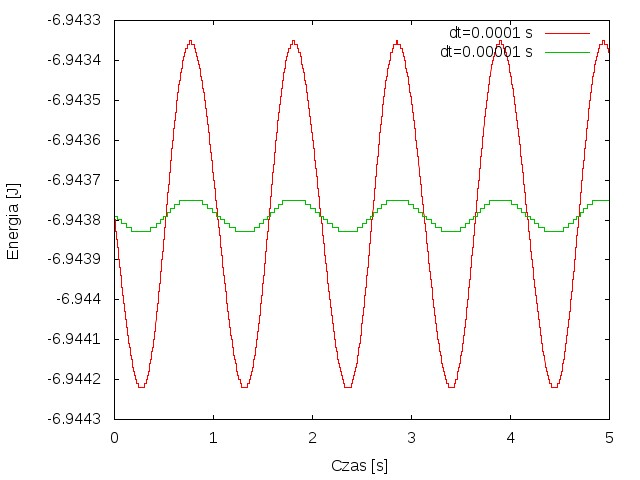
\includegraphics[width=0.6\textwidth]{eng.jpg}
\caption{Wahania całkowitej energii układu dla dwóch różnych kroków czasowych.}
\label{E}
\end{figure}

Na wykresie \ref{M1} zaprezentowano wyniki symulacji $\varphi = \varphi (t)$ dla różnych wychyleń początkowych. 
Można zauważyć, że dla małych amplitud krzywa przechodzi w kosinus, natomiast dla tychże dążących do $\pi$ przechodzi 
w funkcję schodkową.

Na wykresach \ref{M2} zaprezentowano porównanie wyników symulacji z rozwiązaniem analitycznym o którym mowa we wstępie.
Jak można się było spodziewać krzywe nie pokrywają się dla dużych amplitud, gdyż tam nie jest spełnione przybliżenie 
$\sin \varphi \simeq \varphi.$ Natomiast dla amplitudy równej 0.1 mamy już całkowitą zgodność.

\begin{figure}[h!]
\centering
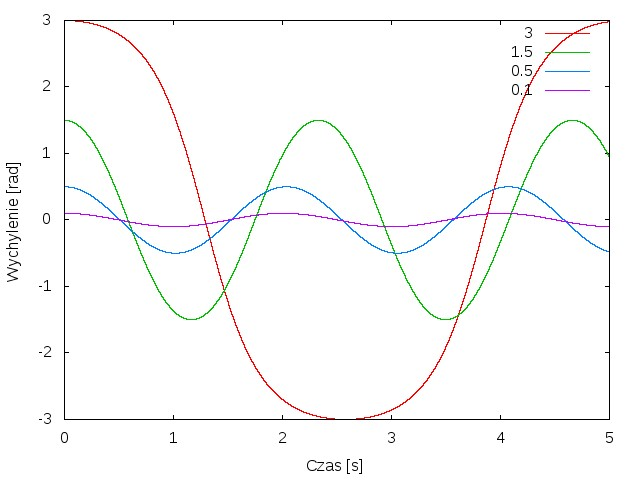
\includegraphics[width=0.6\textwidth]{multi2.jpg}
\caption{Wykresy uzyskanych numerycznie funkcji $\varphi (t)$ dla 
różnych wychyleń początkowych (podanych w radianach).}
\label{M1}
\end{figure}

\begin{figure}[h!]
\centering
\subfloat[$A$=3]{\label{M21}
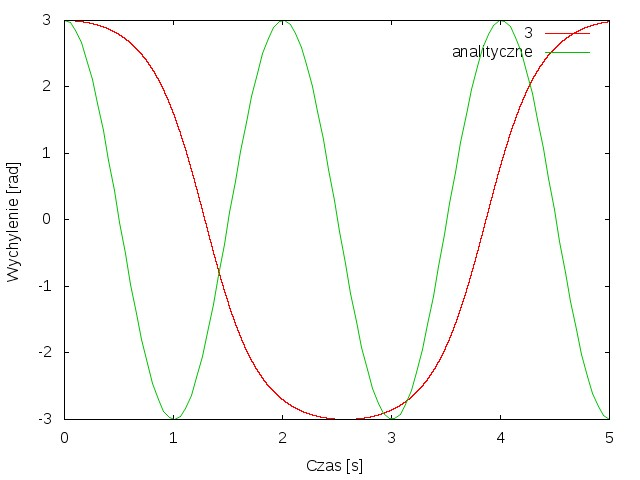
\includegraphics[width=0.4\textwidth]{noan.jpg}}
\quad
\subfloat[$A$=1,5]{\label{M22}
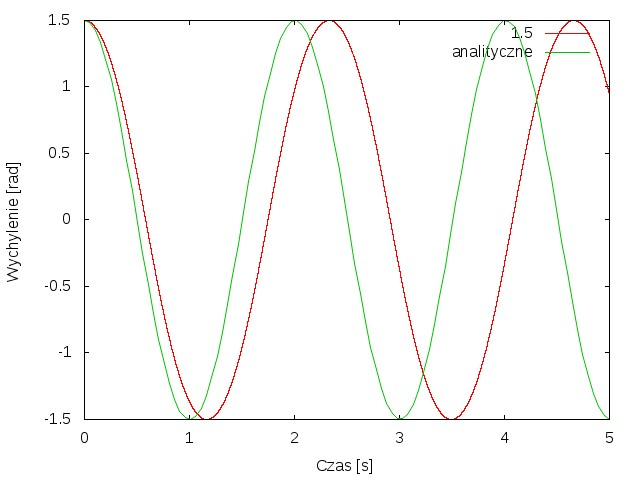
\includegraphics[width=0.4\textwidth]{lian.jpg}}
\quad
\subfloat[$A$=0,5]{\label{M23}
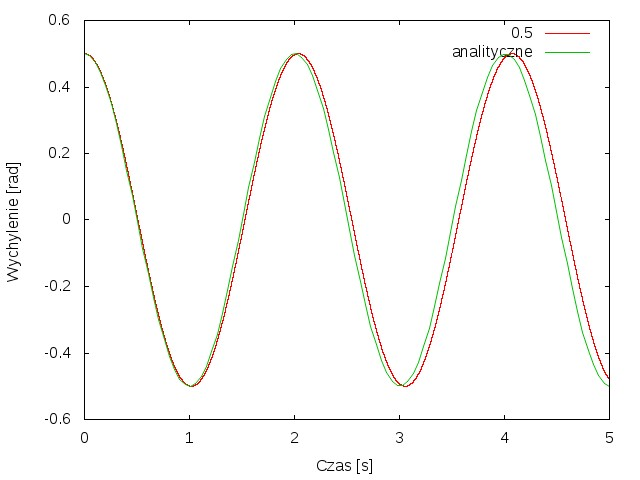
\includegraphics[width=0.4\textwidth]{close.jpg}}
\quad
\subfloat[$A$=0,1]{\label{M24}
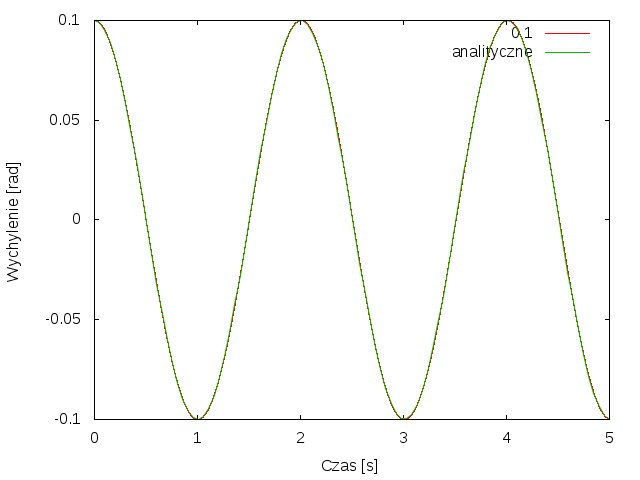
\includegraphics[width=0.4\textwidth]{pro.jpg}}
\caption{Porównanie rozwiązania uzyskanego numerycznie do 
przybliżenia analitycznego (\ref{3}) przy różnych wychyleniach początkowych.}
\label{M2}
\end{figure}
Następnie zbadano zależność okresu wahnięcia od amplitudy. Wyniki przedstawiono na wykresie \ref{T}. Można zauważyć, że dla
małych wychyleń ($<0.4$) okres jest właściwie stały. Natomiast dla faz początkowych bliskich $\pi$ szybko rośnie do 
nieskończoności. Sytuacja $\varphi(0) = \pi$ odpowiada postawieniu wahadła na sztorc, mamy więc sytuację \underline{równowagi} chwiejnej co
sprowadza się do braku drgań.
\begin{figure}[h!]
\centering
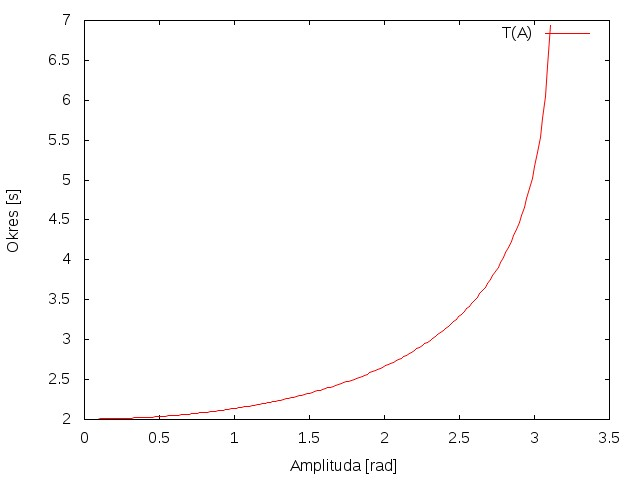
\includegraphics[width=0.6\textwidth]{okres.jpg}
\caption{Zależność okresu wahania od wychylenia początkowego (amplitudy).}
\label{T}
\end{figure}

\section*{Podsumowanie}
W rozważanym tu ruchu, mimo jego dużej prostoty, nie da się uzyskać ogólnego rozwiązania analitycznego, a jedynie przybliżenie dla małych kątów.
Problem ten można jednak w dosyć prosty sposób rozwiązać numerycznie uzyskując dla małych kątów bardzo dobrą zgodność z drogą analityczną, natomiast 
dla pozostałych sensowne wyniki. Uzyskano również zależność okresu od amplitudy. Dla małych kątów można go przybliżyć funkcją stałą, natomiast dla dużych gwałtownie rośnie.


\end{document}


